\documentclass{beamer}
\usepackage{hyperref}
\usepackage{iftex}

% ===========================================================================
% Citations (biblatex with footnote style)
% ===========================================================================
\usepackage[backend=biber,style=verbose,autocite=footnote,maxbibnames=2]{biblatex}
\addbibresource{ref/refs.bib}
\renewcommand{\footnotesize}{\scriptsize}
\setbeamertemplate{bibliography item}{}
\renewcommand*{\bibfont}{\scriptsize}

% ===========================================================================
% Font setup  (Lexend / Inter — bundled in fonts/)
% ===========================================================================
\ifPDFTeX
  \usepackage[sfdefault]{inter}
\else
  \usepackage{fontspec}
  \defaultfontfeatures{Ligatures=TeX, Scale=MatchLowercase}

  \IfFileExists{fonts/Lexend/Lexend-Regular.ttf}{
    \setmainfont{Lexend-Regular.ttf}[
      Path = fonts/Lexend/,
      UprightFont  = Lexend-Regular.ttf,
      BoldFont     = Lexend-Bold.ttf,
      ItalicFont   = Lexend-Regular.ttf,
      BoldItalicFont = Lexend-Bold.ttf,
      ItalicFeatures     = {FakeSlant=0.2},
      BoldItalicFeatures = {FakeSlant=0.2}
    ]
    \setsansfont{Lexend-Regular.ttf}[
      Path = fonts/Lexend/,
      UprightFont  = Lexend-Regular.ttf,
      BoldFont     = Lexend-Bold.ttf,
      ItalicFont   = Lexend-Regular.ttf,
      BoldItalicFont = Lexend-Bold.ttf,
      ItalicFeatures     = {FakeSlant=0.2},
      BoldItalicFeatures = {FakeSlant=0.2}
    ]
  }{
    \IfFontExistsTF{Lexend}{
      \setmainfont{Lexend}
      \setsansfont{Lexend}
    }{}
  }

  \renewcommand{\familydefault}{\sfdefault}

  \IfFileExists{fonts/Inter/Inter-Regular.ttf}{
    \newfontfamily\Inter{Inter-Regular.ttf}[
      Path       = fonts/Inter/,
      UprightFont  = Inter-Regular.ttf,
      ItalicFont   = Inter-Italic.ttf,
      BoldFont     = Inter-Bold.ttf,
      BoldItalicFont = Inter-BoldItalic.ttf
    ]
    \newcommand{\inter}[1]{{\Inter ##1}}
  }{
    \IfFontExistsTF{Inter}{
      \newfontfamily\Inter{Inter}
      \newcommand{\inter}[1]{{\Inter ##1}}
    }{
      \newcommand{\inter}[1]{##1}
    }
  }

  \ifXeTeX
    \usepackage{xeCJK}
    \IfFileExists{C:/Windows/Fonts/msyh.ttc}{
      \setCJKmainfont{msyh.ttc}[
        Path = C:/Windows/Fonts/,
        BoldFont = msyhbd.ttc,
        ItalicFont = msyh.ttc,
        BoldItalicFont = msyhbd.ttc,
        ItalicFeatures = {FakeSlant=0.2},
        BoldItalicFeatures = {FakeSlant=0.2}
      ]
      \setCJKsansfont{msyh.ttc}[
        Path = C:/Windows/Fonts/,
        BoldFont = msyhbd.ttc,
        ItalicFont = msyh.ttc,
        BoldItalicFont = msyhbd.ttc,
        ItalicFeatures = {FakeSlant=0.2},
        BoldItalicFeatures = {FakeSlant=0.2}
      ]
      \setCJKmonofont{msyh.ttc}[Path = C:/Windows/Fonts/]
    }{
      \IfFontExistsTF{Microsoft YaHei}{
        \setCJKmainfont{Microsoft YaHei}[ItalicFont=*,ItalicFeatures={FakeSlant=0.2}]
        \setCJKsansfont{Microsoft YaHei}[ItalicFont=*,ItalicFeatures={FakeSlant=0.2}]
      }{
        \IfFontExistsTF{SimSun}{
          \setCJKmainfont{SimSun}
        }{}
      }
    }
  \fi
\fi

% ===========================================================================
% Colours
% ===========================================================================
\usepackage{xcolor}
\definecolor{mycolor}{RGB}{219, 232, 251}
\definecolor{SYSUGreen}{RGB}{0, 88, 38}
\definecolor{SYSUGreenLight}{RGB}{230, 240, 235}
\definecolor{SYSUGreenMid}{RGB}{51, 121, 81}
\definecolor{SYSUGreenDark}{RGB}{0, 61, 27}
\definecolor{AccentBlue}{RGB}{0, 102, 204}
\definecolor{LightGray}{RGB}{245, 245, 245}
\definecolor{DarkGray}{RGB}{80, 80, 80}

% ===========================================================================
% Packages
% ===========================================================================
\usepackage{latexsym,amsmath,xcolor,multicol,booktabs,calligra}
\usepackage{graphicx,pstricks,listings,stackengine}
\usepackage{multirow}
\usepackage{tikz}
\usepackage{pifont}
\usetikzlibrary{shapes.geometric, arrows.meta, shadows, positioning, calc}

% ===========================================================================
% Beamer font / colour overrides
% ===========================================================================
\setbeamerfont{section in toc}{size=\normalsize,series=\bfseries}
\setbeamerfont{subsection in toc}{size=\small}

% --- Fill in your info here ------------------------------------------------
\newcommand{\authorname}{Your Name}          % <-- change this
\newcommand{\institutename}{Sun Yat-sen University} % <-- and this
\newcommand{\supervisorname}{刘教授}
\author[\authorname]{\authorname}
\title[Short Title]{Your Presentation Title}
\institute{\institutename}
\date{\today}
% ---------------------------------------------------------------------------

\usepackage{SYSU}

\AtBeginSubsection[]{}

% Section divider pages
\makeatletter
\newcounter{majorsection}
\setcounter{majorsection}{0}
\AtBeginSection[]{%
  \stepcounter{majorsection}%
  \ifnum\value{majorsection}>0%
    \begin{frame}[plain]
      \vspace{0.8cm}
      \begin{center}
        {\color{SYSUGreen}\rule{0.85\textwidth}{1.2pt}}\\[0.6cm]
        {\LARGE\bfseries \insertsection}\\[0.45cm]
        {\color{SYSUGreen}\rule{0.85\textwidth}{1.2pt}}
      \end{center}
      \vfill
      \begin{center}
        {\small\color{DarkGray}\authorname\hspace{0.9em}\textbar\hspace{0.9em}\institutename}
      \end{center}
      \vspace{0.2cm}
    \end{frame}
  \fi
}
\makeatother

% Image search paths
\graphicspath{{pic/}}

% ===========================================================================
% Code listings style
% ===========================================================================
\definecolor{deepblue}{rgb}{0,0,0.5}
\definecolor{deepred}{rgb}{0.6,0,0}
\definecolor{deepgreen}{rgb}{0,0.5,0}
\definecolor{halfgray}{gray}{0.55}

\lstset{
    basicstyle=\ttfamily\small,
    keywordstyle=\bfseries\color{deepblue},
    emphstyle=\ttfamily\color{deepred},
    stringstyle=\color{deepgreen},
    numbers=left,
    numberstyle=\tiny\color{halfgray},
    rulesepcolor=\color{red!20!green!20!blue!20},
    frame=single,
    frameround=tttt,
    backgroundcolor=\color{LightGray},
    xleftmargin=1.5em,
    framexleftmargin=1.5em,
    breaklines=true,
    breakatwhitespace=true,
    tabsize=2,
}

% ===========================================================================
% Beamer item / block styling
% ===========================================================================
\setbeamertemplate{itemize items}[circle]
\setbeamercolor{itemize item}{fg=AccentBlue}
\setbeamercolor{itemize subitem}{fg=AccentBlue}
\setbeamercolor{enumerate item}{fg=AccentBlue}

\setbeamercolor{block title}{bg=AccentBlue!10,fg=AccentBlue}
\setbeamercolor{block body}{bg=LightGray,fg=black}

\setbeamercolor{section in toc}{fg=AccentBlue}
\setbeamercolor{subsection in toc}{fg=DarkGray}
\setbeamercolor{section in toc shaded}{fg=DarkGray!50}
\setbeamertemplate{section in toc}[sections numbered]
\setbeamertemplate{subsection in toc}[subsections numbered]

% Fancy placeholder box (use \placeholder{text} for draft slides)
\newcommand{\placeholder}[1]{%
    \begin{center}
    \begin{tikzpicture}
        \node[rectangle, rounded corners=5pt, draw=AccentBlue, line width=1.5pt,
              fill=mycolor, text width=0.75\textwidth, align=center,
              minimum height=3cm, drop shadow] {%
            \textcolor{AccentBlue}{\textbf{#1}}
        };
    \end{tikzpicture}
    \end{center}
}


\begin{document}

%=============================================================================
% Title Page
%=============================================================================
{%
  \title[Short Title]%
        {Your Presentation Title\\with a Subtitle Line}
  \author[\authorname]{\authorname\hspace{0.9em}\textbar\hspace{0.9em}\today}
  \institute[\institutename]{\institutename\\ Supervisor: \supervisorname}
  \date{}
  \titlegraphic{
\includegraphics[width=0.18\linewidth]{sysu_logo.png}}
  \begin{frame}
      \titlepage
  \end{frame}
}%

%=============================================================================
% Outline
%=============================================================================
\begin{frame}{Outline}
    \vspace{0.2cm}
    \begin{enumerate}
        \setlength{\itemsep}{0.7em}
        \item Introduction \& Motivation
        \item Methodology
        \item Experiments \& Results
        \item Case Study
        \item Conclusion \& Future Work
    \end{enumerate}
\end{frame}

%=============================================================================
% Section 1: Introduction
%=============================================================================
\section[Introduction]{Introduction \& Motivation}

\begin{frame}{Background}
    \begin{itemize}
        \setlength{\itemsep}{0.6em}
        \item Deep learning has achieved remarkable success across many domains\footfullcite{lecun2015deep}
        \item The Transformer architecture revolutionised sequence modelling\footfullcite{vaswani2017attention}
        \item Pre-trained language models further advanced NLP capabilities\footfullcite{devlin2019bert}
    \end{itemize}
\end{frame}

\begin{frame}{Research Question}
    \begin{block}{Core Question}
        \centering
        \large \textit{How can we improve X while maintaining Y under constraint Z?}
    \end{block}
    \vspace{0.4cm}
    \begin{itemize}
        \setlength{\itemsep}{0.7em}
        \item \textcolor{AccentBlue}{\textbf{Challenge 1}}: Existing methods overlook cross-layer interactions
        \item \textcolor{AccentBlue}{\textbf{Challenge 2}}: Scalability remains an open issue for large models
        \item \textcolor{AccentBlue}{\textbf{Our approach}}: A unified framework that addresses both challenges
    \end{itemize}
\end{frame}

%=============================================================================
% Section 2: Methodology
%=============================================================================
\section[Methodology]{Methodology}

\begin{frame}{Method Overview}
    \begin{columns}
        \column{0.55\textwidth}
        \begin{itemize}
            \setlength{\itemsep}{0.55em}
            \item \textbf{Step 1}: Collect observations and build feature matrix \(X\)
            \item \textbf{Step 2}: Factorise \(X \approx DR\) to discover latent patterns
            \item \textbf{Step 3}: Apply sparsity constraints for interpretability
        \end{itemize}
        \column{0.42\textwidth}
        \begin{center}
            % TikZ inline figure — replace with your own image
            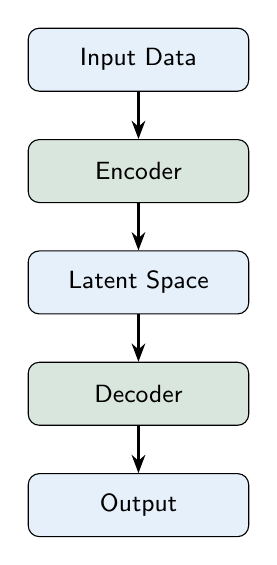
\begin{tikzpicture}[scale=0.65, every node/.style={font=\small}]
                \node[draw, rounded corners, fill=AccentBlue!10, minimum width=2.8cm, minimum height=0.8cm] (input) {Input Data};
                \node[draw, rounded corners, fill=SYSUGreen!15, minimum width=2.8cm, minimum height=0.8cm, below=0.6cm of input] (enc) {Encoder};
                \node[draw, rounded corners, fill=AccentBlue!10, minimum width=2.8cm, minimum height=0.8cm, below=0.6cm of enc] (latent) {Latent Space};
                \node[draw, rounded corners, fill=SYSUGreen!15, minimum width=2.8cm, minimum height=0.8cm, below=0.6cm of latent] (dec) {Decoder};
                \node[draw, rounded corners, fill=AccentBlue!10, minimum width=2.8cm, minimum height=0.8cm, below=0.6cm of dec] (output) {Output};
                \draw[-{Stealth}, thick] (input) -- (enc);
                \draw[-{Stealth}, thick] (enc) -- (latent);
                \draw[-{Stealth}, thick] (latent) -- (dec);
                \draw[-{Stealth}, thick] (dec) -- (output);
            \end{tikzpicture}
        \end{center}
    \end{columns}
\end{frame}

\begin{frame}{Mathematical Formulation}
    \begin{block}{Objective function}
        \[
        \mathcal{L}(D,R)=\underbrace{\|X - DR\|_F^2}_{\text{reconstruction}}
        +\lambda_1 \underbrace{\|R\|_1}_{\text{sparsity}}
        +\lambda_2 \underbrace{\Omega(D)}_{\text{regularisation}}
        \]
    \end{block}
    \vspace{0.2cm}
    \begin{itemize}
        \setlength{\itemsep}{0.5em}
        \item \(X \in \mathbb{R}^{m \times n}\): observation matrix (features \(\times\) samples)
        \item \(D \in \mathbb{R}^{m \times k}\): dictionary of \(k\) latent patterns
        \item \(R \in \mathbb{R}^{k \times n}\): sparse representation coefficients
        \item \(\lambda_1, \lambda_2\): trade-off hyper-parameters
    \end{itemize}
\end{frame}

\begin{frame}{Algorithm: Alternating Optimisation}
    \begin{enumerate}
        \setlength{\itemsep}{0.7em}
        \item \textcolor{AccentBlue}{\textbf{Initialise}} \(D^{(0)}\) randomly; set \(t=0\)
        \item \textcolor{AccentBlue}{\textbf{Repeat}} until convergence:
        \begin{enumerate}
            \item Fix \(D^{(t)}\), solve for \(R^{(t+1)}\) via LASSO
            \item Fix \(R^{(t+1)}\), update \(D^{(t+1)}\) via projected gradient descent
            \item \(t \leftarrow t + 1\)
        \end{enumerate}
        \item \textcolor{AccentBlue}{\textbf{Return}} \(D^{(t)}\), \(R^{(t)}\)
    \end{enumerate}
    \vspace{0.3cm}
    \begin{alertblock}{Complexity}
        Per-iteration cost: \(\mathcal{O}(mnk)\). Typical convergence in 50--200 iterations.
    \end{alertblock}
\end{frame}

%=============================================================================
% Section 3: Experiments & Results
%=============================================================================
\section[Results]{Experiments \& Results}

\begin{frame}{Experimental Setup}
    \begin{itemize}
        \setlength{\itemsep}{0.7em}
        \item \textcolor{AccentBlue}{\textbf{Models}}: ModelA-Base, ModelB-Large
        \item \textcolor{AccentBlue}{\textbf{Datasets}}: CIFAR-100, ImageNet-1K, GLUE benchmark
        \item \textcolor{AccentBlue}{\textbf{Hardware}}: 4\(\times\) NVIDIA A100 80GB
        \item \textcolor{AccentBlue}{\textbf{Training}}: 100 epochs, AdamW optimiser, cosine LR schedule
        \item \textcolor{AccentBlue}{\textbf{Evaluation}}: Top-1 accuracy, F1 score, inference latency
    \end{itemize}
\end{frame}

\begin{frame}{Main Results (Higher is Better)}
    \centering
    \scriptsize
    \begin{tabular}{l|lccccc}
        \toprule
        \textbf{Model} & \textbf{Method} & \textbf{AVG} & \textbf{Task A} & \textbf{Task B} & \textbf{Task C} & \textbf{Task D} \\
        \midrule
        \multirow{4}{*}{ModelA}
        & Full Model   & 0.892 & 0.921 & 0.873 & 0.901 & 0.872 \\
        & Baseline-1   & 0.826 & 0.854 & 0.812 & 0.835 & 0.805 \\
        & Baseline-2   & 0.838 & 0.861 & 0.825 & 0.842 & 0.823 \\
        & \textbf{Ours} & \textbf{0.867} & \textbf{0.893} & \textbf{0.851} & \textbf{0.871} & \textbf{0.854} \\
        \midrule
        \multirow{4}{*}{ModelB}
        & Full Model   & 0.905 & 0.932 & 0.889 & 0.912 & 0.886 \\
        & Baseline-1   & 0.841 & 0.870 & 0.824 & 0.851 & 0.818 \\
        & Baseline-2   & 0.856 & 0.879 & 0.841 & 0.863 & 0.840 \\
        & \textbf{Ours} & \textbf{0.881} & \textbf{0.908} & \textbf{0.867} & \textbf{0.885} & \textbf{0.865} \\
        \bottomrule
    \end{tabular}

    \vspace{0.4cm}
    \normalsize
    \begin{itemize}
        \item \textcolor{AccentBlue}{\textbf{Takeaway}}: Our method consistently outperforms both baselines
        \item The gap is more pronounced on harder tasks (Task B, Task D)
    \end{itemize}
\end{frame}

\begin{frame}{Ablation Study}
    \centering
    \scriptsize
    \begin{tabular}{lcccc}
        \toprule
        \textbf{Variant} & \textbf{Accuracy} & \textbf{F1} & \textbf{Latency (ms)} & \textbf{Parameters (M)} \\
        \midrule
        Full method          & \textbf{0.881} & \textbf{0.874} & 12.3 & 125  \\
        w/o sparsity         & 0.862 & 0.854 & 12.1 & 125  \\
        w/o regularisation   & 0.871 & 0.863 & 12.4 & 125  \\
        Smaller dictionary   & 0.855 & 0.847 & \textbf{9.8}  & \textbf{98}   \\
        Larger dictionary    & 0.879 & 0.873 & 15.7 & 152  \\
        \bottomrule
    \end{tabular}
    \vspace{0.3cm}
    \normalsize
    \begin{itemize}
        \item Both sparsity and regularisation contribute to performance
        \item Dictionary size offers an accuracy--efficiency trade-off
    \end{itemize}
\end{frame}

%=============================================================================
% Section 4: Case Study
%=============================================================================
\section[Case Study]{Case Study}

\begin{frame}{Visualisation: Learned Patterns}
    \begin{columns}
        \column{0.52\textwidth}
        \begin{itemize}
            \setlength{\itemsep}{0.6em}
            \item Each column of \(D\) corresponds to a latent pattern
            \item Semantically similar inputs activate overlapping patterns
            \item Patterns form a meaningful hierarchy: fine-grained \(\to\) coarse-grained
        \end{itemize}
        \column{0.45\textwidth}
        \begin{center}
            % Example TikZ heatmap-style visualisation
            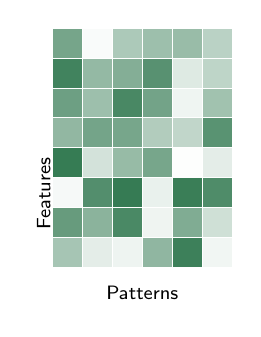
\begin{tikzpicture}[scale=0.38]
                \foreach \y in {0,...,7} {
                    \foreach \x in {0,...,5} {
                        \pgfmathsetmacro{\val}{rnd*100}
                        \pgfmathsetmacro{\clr}{\val/100*80}
                        \fill[SYSUGreen!\clr] (\x,\y) rectangle (\x+1,\y+1);
                        \draw[white, very thin] (\x,\y) rectangle (\x+1,\y+1);
                    }
                }
                \node[below, font=\scriptsize] at (3,-0.3) {Patterns};
                \node[left, font=\scriptsize, rotate=90] at (-0.3,4) {Features};
            \end{tikzpicture}
        \end{center}
    \end{columns}
\end{frame}

\begin{frame}{TikZ Flowchart Example}
    \begin{center}
    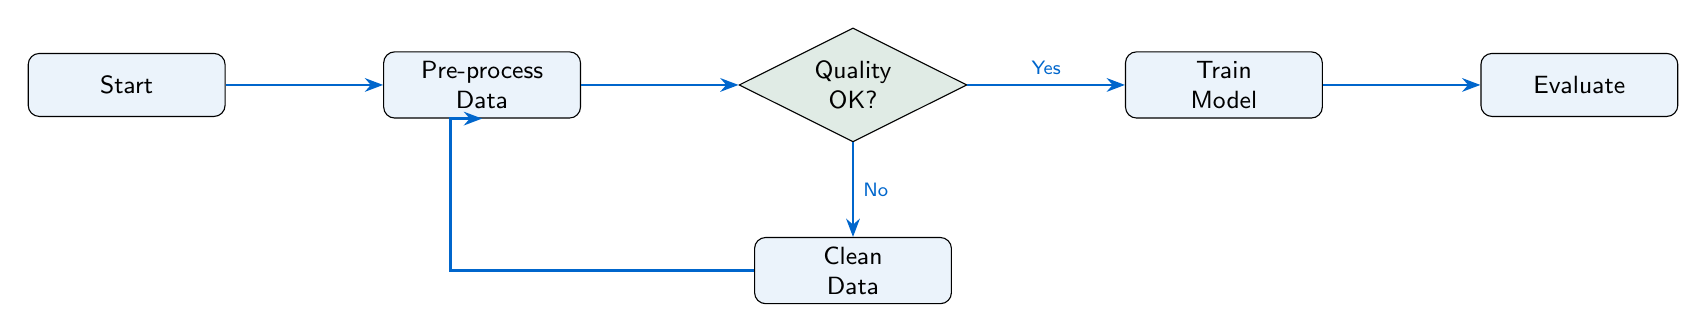
\begin{tikzpicture}[
        node distance=1.2cm and 2cm,
        box/.style={draw, rounded corners, fill=AccentBlue!8,
                    minimum width=2.5cm, minimum height=0.8cm,
                    font=\small, align=center},
        decision/.style={draw, diamond, fill=SYSUGreen!12,
                    minimum width=1.5cm, minimum height=0.8cm,
                    font=\small, align=center, aspect=2},
        arr/.style={-{Stealth}, thick, AccentBlue}
    ]
        \node[box] (start) {Start};
        \node[box, right=of start] (proc1) {Pre-process\\Data};
        \node[decision, right=of proc1] (dec1) {Quality\\OK?};
        \node[box, right=of dec1] (proc2) {Train\\Model};
        \node[box, below=of dec1] (fix) {Clean\\Data};
        \node[box, right=of proc2] (end) {Evaluate};

        \draw[arr] (start) -- (proc1);
        \draw[arr] (proc1) -- (dec1);
        \draw[arr] (dec1) -- node[above]{\scriptsize Yes} (proc2);
        \draw[arr] (dec1) -- node[right]{\scriptsize No} (fix);
        \draw[arr] (fix.west) -| ([xshift=-0.4cm]proc1.south) -- (proc1.south);
        \draw[arr] (proc2) -- (end);
    \end{tikzpicture}
    \end{center}
\end{frame}

\begin{frame}[fragile]{Code Listing Example}
    \begin{lstlisting}[language=Python, caption={Training loop (simplified)}]
import torch
import torch.nn as nn

model = MyModel(hidden_dim=256, n_layers=6)
optimizer = torch.optim.AdamW(model.parameters(), lr=3e-4)
criterion = nn.CrossEntropyLoss()

for epoch in range(100):
    for batch in dataloader:
        x, y = batch
        logits = model(x)
        loss = criterion(logits, y)
        loss.backward()
        optimizer.step()
        optimizer.zero_grad()
    print(f"Epoch {epoch}: loss={loss.item():.4f}")
    \end{lstlisting}
\end{frame}

\begin{frame}{Using Columns \& Images Together}
    \begin{columns}
        \column{0.55\textwidth}
        \begin{itemize}
            \setlength{\itemsep}{0.55em}
            \item Left column for text explanations
            \item Right column for figures or diagrams
            \item Adjust \texttt{column} widths to taste
        \end{itemize}
        \vspace{0.3cm}
        \begin{exampleblock}{Tip}
            Use \texttt{\textbackslash placeholder\{text\}} during drafting to reserve space for future figures.
        \end{exampleblock}
        \column{0.42\textwidth}
        \placeholder{Your figure here}
    \end{columns}
\end{frame}

\begin{frame}{Multi-Column Layout}
    \begin{multicols}{2}
        \textbf{Advantages}
        \begin{itemize}
            \item Fast convergence
            \item Low memory footprint
            \item Easy to parallelise
        \end{itemize}
        \columnbreak
        \textbf{Limitations}
        \begin{itemize}
            \item Sensitive to initialisation
            \item Requires tuning \(\lambda\)
            \item Limited to linear decomposition
        \end{itemize}
    \end{multicols}
    \vspace{0.3cm}
    \begin{block}{Summary}
        The method works best when the underlying structure is approximately low-rank and sparse.
    \end{block}
\end{frame}

%=============================================================================
% Section 5: Conclusion
%=============================================================================
\section[Conclusion]{Conclusion \& Future Work}

\begin{frame}{Conclusion}
    \begin{itemize}
        \setlength{\itemsep}{0.8em}
        \item \textcolor{AccentBlue}{\textbf{Contribution 1}}: We proposed a novel framework for discovering latent structures
        \item \textcolor{AccentBlue}{\textbf{Contribution 2}}: Our approach achieves state-of-the-art results while remaining interpretable
        \item \textcolor{AccentBlue}{\textbf{Contribution 3}}: Open-source tooling for interactive exploration
    \end{itemize}
    \vspace{0.4cm}
    \begin{block}{Future directions}
        \begin{itemize}
            \item Extend to non-linear decomposition methods
            \item Scale to billion-parameter models
            \item Integrate with continual learning settings
        \end{itemize}
    \end{block}
\end{frame}

\begin{frame}{}
    \vspace{1.5cm}
    \begin{center}
        {\Huge\bfseries Thank You!}\\[0.8cm]
        {\Large Questions are welcome.}\\[1cm]
        {\normalsize
            \textcolor{AccentBlue}{\textbf{Email}}: your.email@mail.sysu.edu.cn\\[0.3cm]
            \textcolor{AccentBlue}{\textbf{GitHub}}: \url{https://github.com/your-username}
        }
    \end{center}
\end{frame}

\begin{frame}[allowframebreaks]{References}
    \setbeamertemplate{bibliography item}{}
    \printbibliography[heading=none]
\end{frame}

\end{document}
